% File: Rolling.tex
% Author: Adam Leeper
%------------------------------------------------------------------------------
\providecommand{\isolatedBuild}[1]{#1}% Fallback definition to build normally.
\isolatedBuild{
  \documentclass[11pt,letterpaper]{book}
  %\documentclass[11pt,letterpaper]{book}

% aleeper: I think these are needed for Paul's macros?
\usepackage{epsfig}
\usepackage{epstopdf}

%\makeatletter
%\typeout{The import path is \import@path}
%\makeatother

\usepackage{import}

\subimport{./}{packagesMitiguy.sty}
\subimport{./}{macrosMitiguy.tex}
\subimport{./}{PageStylesMitiguy.tex}
\subimport{./}{macrosLeeper.tex}
   % Found via TEXINPUTS environment variable.
  \isolatedBuildHeader{Kinetic Energy of Rolling Motion}
                      {Kinetic Energy of Rolling Motion}
}
%%%
%%%
%%%
\begin{minipage}{0.45\textwidth}
  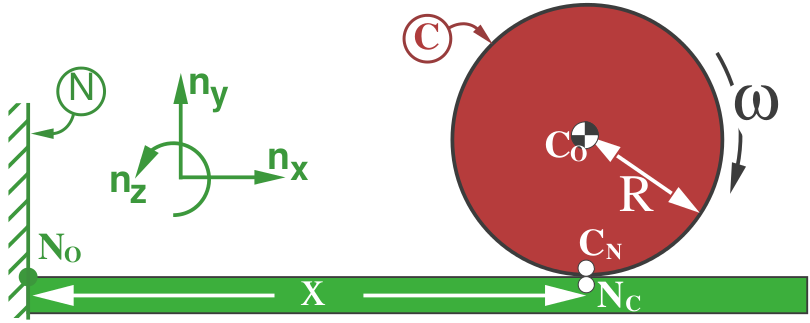
\includegraphics[width=0.95\linewidth]{rolling.png}
\end{minipage}
%
\begin{minipage}{0.45\textwidth}
  A uniform rigid disk \basis{C}, of radius $R$, \textbf{rolls} to the
  \textbf{right} on flat ground (taken to be a Newtonian reference frame
  \basis{N}), with angular velocity $\angvel{C}{N} = -\omega~ \uvecz{n}$.
  You are reminded that, using two-points-fixed, you could find
  $\vel{Ccm}{N} = \omega R~\uvecx{n}$.
\end{minipage}
%
\\[1.0pc]
The formula for kinetic energy of a rigid body $C$ (where $C_p$ is any point
fixed on \basis{C}) is:
$$\ke{C}{N} = \frac{1}{2} ~m^C ~\vel{C_p}{N} \cdot \vel{C_p}{N}
  \plus[\;] \frac{1}{2} ~\angvel{C}{N} \cdot \idyad{C/C_p} \cdot \angvel{C}{N}
  \plus[\;] m^C ~\vel{C_p}{N} \cdot \angvel{C}{N} \times \posvec{C_p}{\cm{C}}$$
%
\begin{enumerate}
  \item First, \textbf{show} that
    % since \basis{B} has a \textit{simple} angular velocity in \basis{N}
    % about \uvecz{b},
    the term
    $(~\frac{1}{2} \angvel{C}{N} \cdot \idyad{C/C_p} \cdot \angvel{C}{N}~)$
    simplifies to
    $(~\frac{1}{2} ~\omega^2 ~\iscalarzz{C/C_p} ~)$ in this case.
    \\[-0.75pc]
    %
  \item Compute \ke{C}{N} when you pick $C_p$ to be \basis{C}'s center of mass,
    \cm{C} (or $C_o$).
    \\[-0.75pc]
    %
  \item Compute \ke{C}{N} when you pick $C_p$ to be the contact point, $C_N$.
\end{enumerate}
%
\textbf{Hint:} You should get the same result in both cases!
\\[1.0pc]
%
\isolatedBuildFooter
